\documentclass[12pt, a4paper]{article}
\usepackage[utf8]{inputenc}
\usepackage[T1]{fontenc}
\usepackage[portuguese]{babel} 
\usepackage{geometry}
\usepackage{graphicx}
\usepackage{tabularx}
\usepackage{booktabs}
\usepackage{float}
\usepackage{parskip}
\usepackage{enumitem}

% Configuração das margens
\geometry{
	top=2.5cm,
	bottom=2.5cm,
	left=2.5cm,
	right=2.5cm
}

\begin{document}
	
	% -------------------------------------------------------------------
	% CAPA (TITLE PAGE)
	% -------------------------------------------------------------------
	\begin{titlepage}
		\centering
		\vspace*{2cm}
		
		{\LARGE \textbf{RNG com não repetição (3 Bits)}}\\[0.5cm]
		{\Huge \textbf{Relatório de síntese}}\\[1.5cm]
		
		{\Large Projeto do Bloco Digital}\\[2cm]
		
		{\Large \textbf{Matheus Grossi}}\\[0.2cm]
		
		\vfill
		
		Data: \today\\
		Rev.: 9.0
		
		\vspace*{1cm}
	\end{titlepage}
	
	% -------------------------------------------------------------------
	% ÍNDICE AUTOMÁTICO
	% -------------------------------------------------------------------
	\tableofcontents
	\vspace*{1cm}
	
	% -------------------------------------------------------------------
	% ACRÓNIMOS
	% -------------------------------------------------------------------
	\section*{Siglas e Acrónimos}
	
	\begin{tabular}{ll}
		\textbf{RNG}  & Random Number Generator (Gerador de Números Aleatórios) \\
		\textbf{PRNG} & Pseudo-Random Number Generator \\
		\textbf{ASIC} & Application Specific Integrated Circuit \\
		\textbf{FPGA} & Field-Programmable Gate Array \\
		\textbf{FSM}  & Finite State Machine (Máquina de Estados Finita) \\
		\textbf{HDL}  & Hardware Description Language \\
		\textbf{RTL}  & Register Transfer Level \\
		\textbf{SDC}  & Synopsys Design Constraints \\
	\end{tabular}
	
	\newpage
	
	% -------------------------------------------------------------------
	% CONTEÚDO PRINCIPAL
	% -------------------------------------------------------------------
	
	\section{Síntese baseada em FPGA}
	Este design é implementado utilizando HDL padrão de indústria e estruturado para facilitar a integração e síntese. 
	
	\begin{itemize}
		\item \textbf{Nome do bloco:} RNG Não Repetitivo (3 bits) 
		\item \textbf{Linguagem de Descrição:} Verilog 
		\item \textbf{Tecnologias Alvo:} FPGA e ASIC 
		\item \textbf{Características Chave:} Interface de Handshake, 4 Seeds, Histórico de não-repetição. 
	\end{itemize}
	
	Abaixo estão as vistas explodidas do design após síntese em FPGA:
	
	\begin{figure}[H]
		\centering
		\fbox{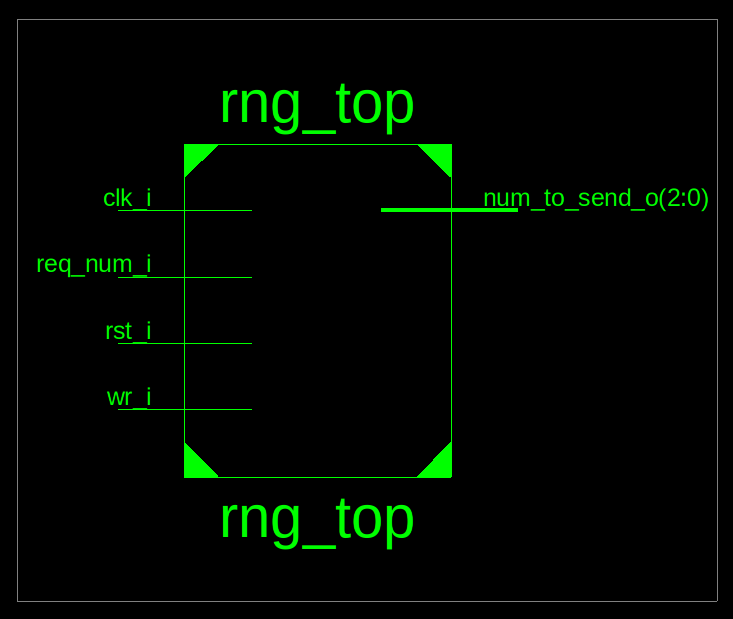
\includegraphics[width=0.65\textwidth]{../../diagrams/fpga_post_synth/top_view.png}}
		\caption{Visão de Topo do Circuito (Síntese)} 
	\end{figure}
	
	% Vistas Explodidas Separadas Verticalmente
	\begin{figure}[H]
		\centering
		\fbox{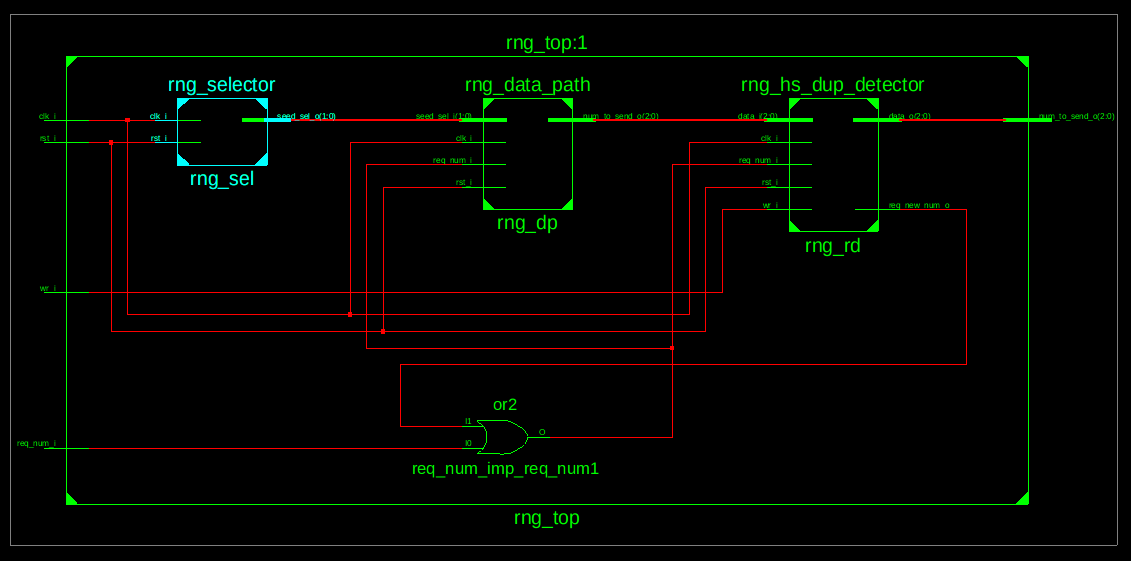
\includegraphics[width=0.65\textwidth]{../../diagrams/fpga_post_synth/xplode_view_pt1.png}}
		\caption{Vista Explodida 1}
	\end{figure}
	
	\begin{figure}[H]
		\centering
		\fbox{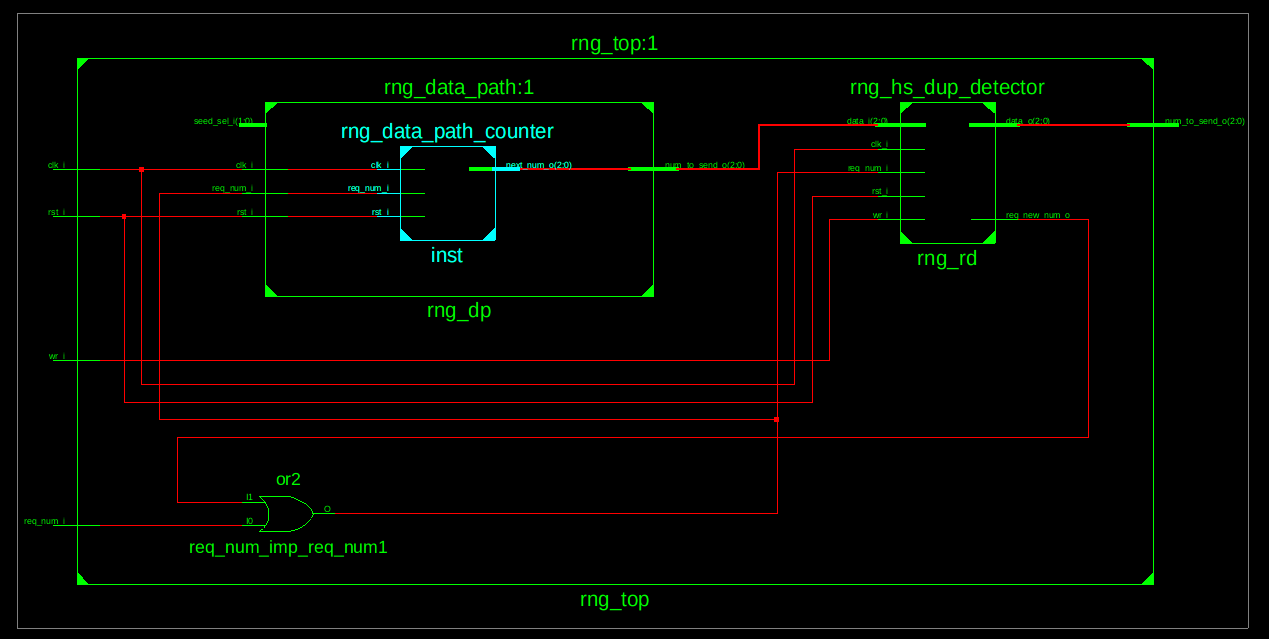
\includegraphics[width=0.65\textwidth]{../../diagrams/fpga_post_synth/xplode_view_pt2.png}}
		\caption{Vista Explodida 2}
	\end{figure}
	
	\begin{figure}[H]
		\centering
		\fbox{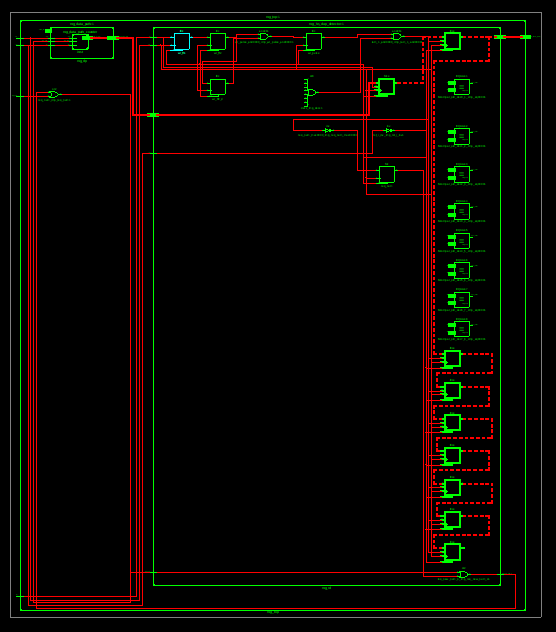
\includegraphics[width=0.85\textwidth]{../../diagrams/fpga_post_synth/xplode_view_pt3.png}}
		\caption{Vista Explodida 3}
	\end{figure}
	
	\begin{figure}[H]
		\centering
		\fbox{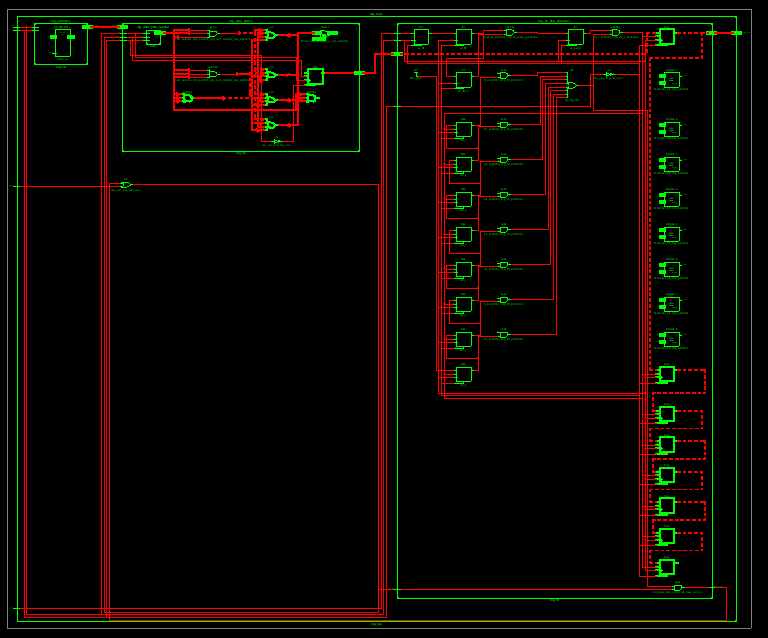
\includegraphics[width=0.95\textwidth]{../../diagrams/fpga_post_synth/xplode_view_pt4.png}}
		\caption{Vista Explodida 4}
	\end{figure}
	
	\section{Fluxo de Funcionamento e Timing}
	O bloco opera através de um fluxo coordenado para garantir a validade dos dados: 
	
	\begin{enumerate}
		\item \textbf{Reset:} O sistema é resetado (\texttt{rst\_i}), limpando a memória do detetor de duplicatas. 
		\item \textbf{Seleção de Seed:} O módulo \texttt{rng\_selector} utiliza um contador \textit{free-running} para definir qual das 4 tabelas será usada. 
		\item \textbf{Geração e Validação:} O \texttt{rng\_data\_path} gera um candidato. O \texttt{rng\_hs\_dup\_detector} verifica duplicatas. Se existir, descarta e busca o próximo. Se for único, disponibiliza na saída. 
		\item \textbf{Confirmação (Handshake):} O sinal \texttt{wr\_i} confirma a leitura e salva o valor no histórico. 
	\end{enumerate}
	
	\begin{figure}[H]
		\centering
		\fbox{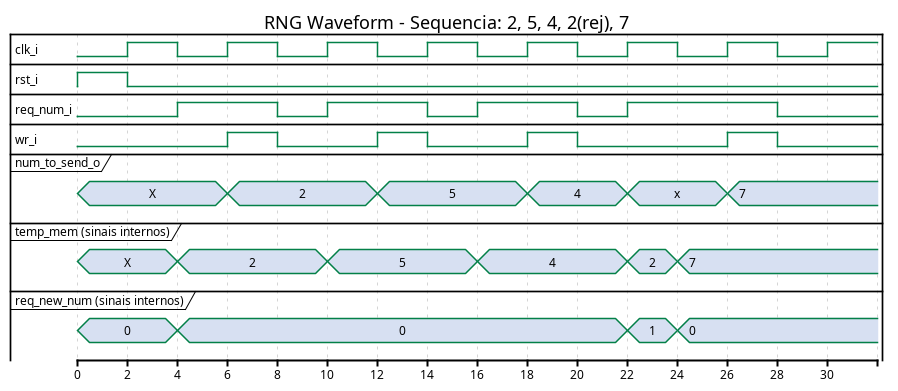
\includegraphics[width=1.0\textwidth]{../../diagrams/timing/timing.png}}
		\caption{Diagrama de Temporização (Timing)} 
		\label{fig:timing}
	\end{figure}
	

	\section{Síntese baseada em ASIC Flow no PDK Open-SKY130}
	
	Além da implementação em FPGA, o projeto foi submetido ao fluxo de design digital para ASIC utilizando o ambiente \textit{Librelane}. O mapeamento tecnológico direcionou o circuito para a biblioteca de \textit{standard cells} de código aberto \texttt{sky130\_fd\_sc\_hd} (SkyWater 130nm High Density). 
	
	\subsection{Definições da estrutura para a síntese}

	Para executar esse processo, siga os passos abaixo:
	\begin{itemize}
		\item Crie uma pasta com o nome do projeto dentro do diretório \texttt{openframe\_user/openlane}.
		\item Internamente a esta pasta, crie um subdiretório chamado \texttt{src}.
		\item Na raiz da pasta do projeto, crie um arquivo nomeado \texttt{config.json}. Este script irá armazenar os dados primários de roteamento e síntese prévios ao SDC.
	\end{itemize}

	\begin{figure}[H]
		\centering
		\fbox{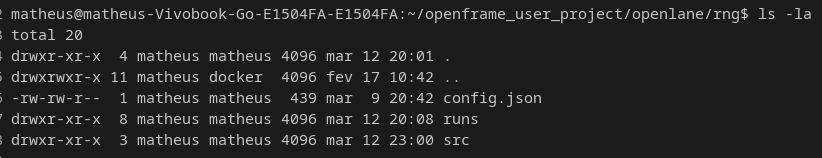
\includegraphics[width=1.0\textwidth]{org.png}}
		\caption{Organzição da pasta de projeto}
		\label{fig:organizacao_da_arv_proj}
	\end{figure}
	
	\begin{itemize}
		\item	Dentro da pasta src insira os arquivos .v e .sv de seu projeto.
		\item	Em meu caso deixei o config.json definido conforme exemplo na pagina oficial do sintetizador.
	\end{itemize}

	\begin{figure}[H]
		\centering
		\fbox{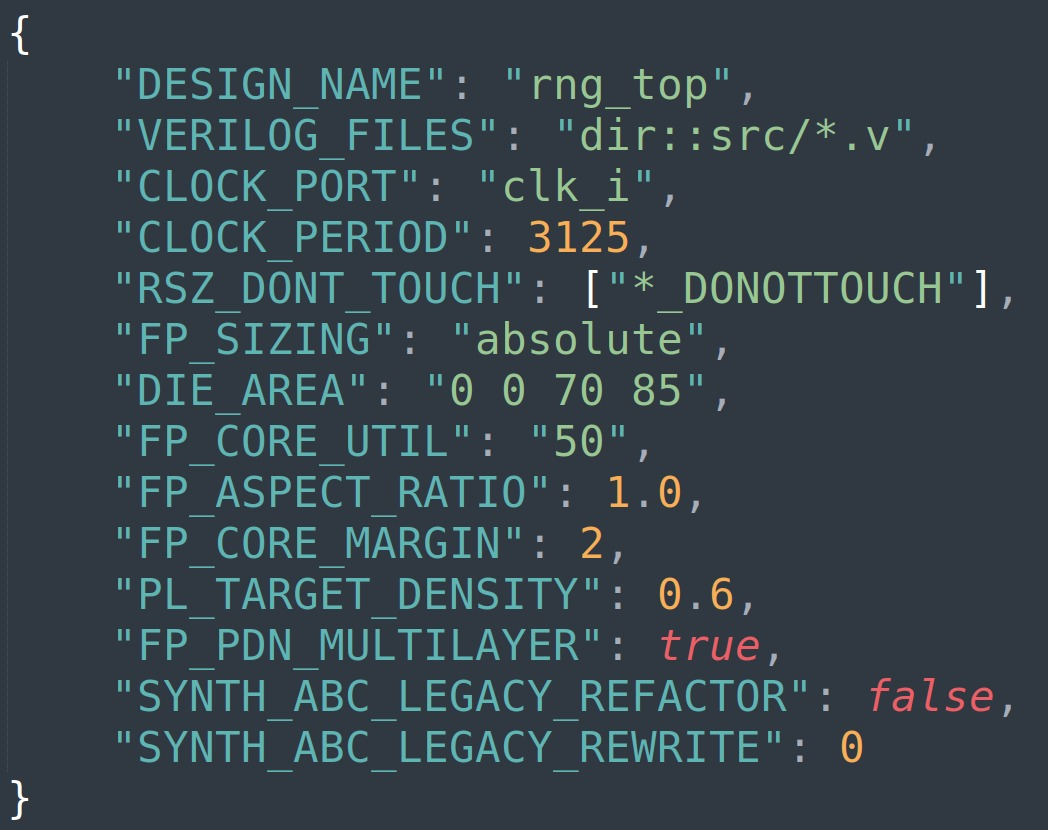
\includegraphics[width=1.0\textwidth]{config.png}}
		\caption{Configuração do script}
		\label{fig:configuracao_do_script}
	\end{figure}

	\subsection{Restrições de Design (SDC - Synopsys Design Constraints)}
	Devido ao fato de este projeto se tratar de uma implementação simples e que não passará por um tape-out foi feito o uso de um SDC genérico, e portanto as constraints usadas foram as padrões, o que implica que as otimizações e temporizações não foram as melhores para esta aplicação
	
	\section{Resultados da Síntese Lógica e Física}
		
	\subsection{Diagrama Lógico}
	A estrutura do módulo \texttt{rng\_top} consolida quatro sub-blocos principais: caminho de dados, seletor de semente, detetor de duplicatas e contador cíclico. 
	A tradução lógica deste caminho de dados para o nível de portas resultou num uso intensivo de multiplexadores para o roteamento e portas exclusivas para validação e contagem. A arquitetura foi sintetizada em 122 células lógicas no total como pode ser observado na imagem abaixo. 
	
	\begin{figure}[H]
		\centering
		\fbox{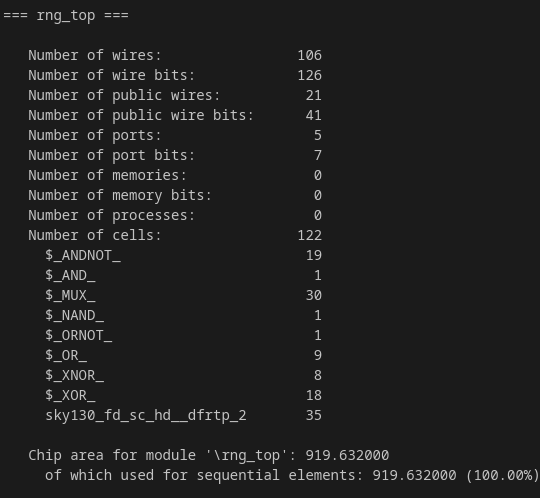
\includegraphics[width=1.0\textwidth]{stats.png}}
		\caption{Composição do SoC}
		\label{fig:comp_soc}
	\end{figure}

	\subsection{Consumo de Potência}
	Os relatórios estáticos de síntese atuais (\texttt{stat.rpt} e \texttt{stat.json}) documentam detalhadamente a área, os tipos de células e as interconexões lógicas. 
	Para avaliar com precisão o consumo de potência estática (\textit{leakage}) e dinâmica, o fluxo requer uma extração pós-roteamento. Esta análise baseia-se na atividade de comutação (\textit{switching activity}), sendo necessário fornecer os ficheiros da simulação (\texttt{.vcd}) gerados em \texttt{waveforms} a uma ferramenta de \textit{Power Analysis} nativa do fluxo Libreane.
	
	\begin{figure}[H]
		\centering
		\fbox{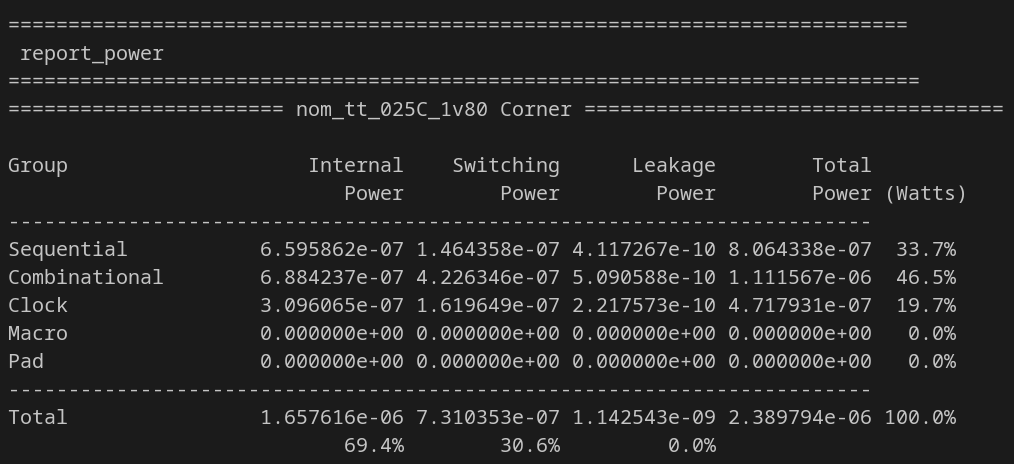
\includegraphics[width=0.9\textwidth]{power.png}}
		\caption{Métricas de Consumo de Potência}
		\label{fig:consumo_potencia}
	\end{figure}
	
	\section{Soc-View}
	Este foi o resultado final de nossa síntese após todos os processos:
	
	\begin{figure}[H]
		\centering
		\fbox{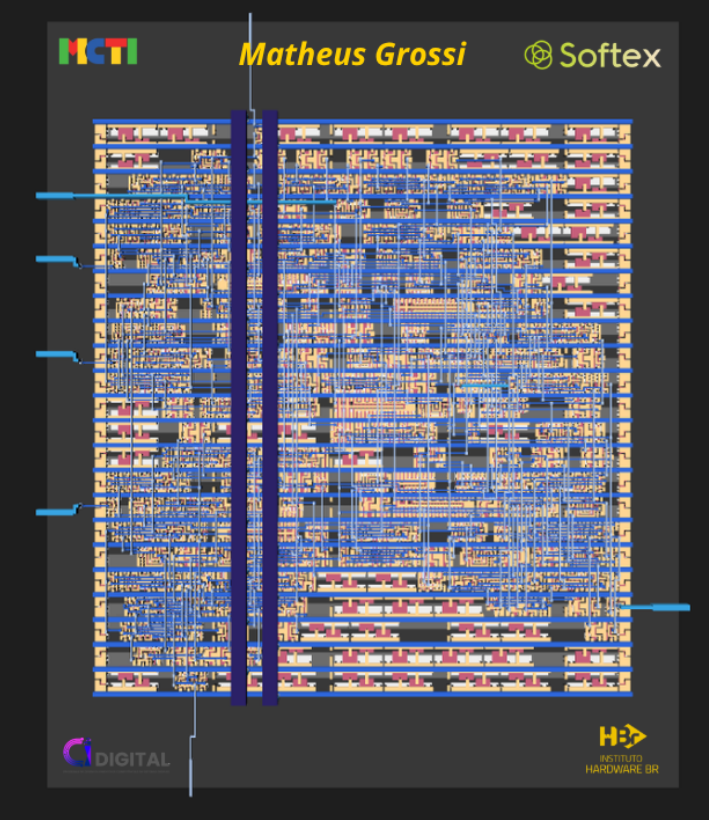
\includegraphics[width=0.7\textwidth]{../../diagrams/soc_view.png}}
		\caption{Waveform da Simulação} 
		\label{fig:waveform}
	\end{figure}

	\section{Simulação}
	Os ambientes de teste estão localizados em \texttt{testbenchs} e utilizam scripts de automação (Makefiles/Bash) para geração de ondas. 
	O waveform abaixo demonstra o comportamento real obtido em simulação com a bancada rodando em nossa netlist pós-síntese. 
	
	\begin{figure}[H]
		\centering
		\fbox{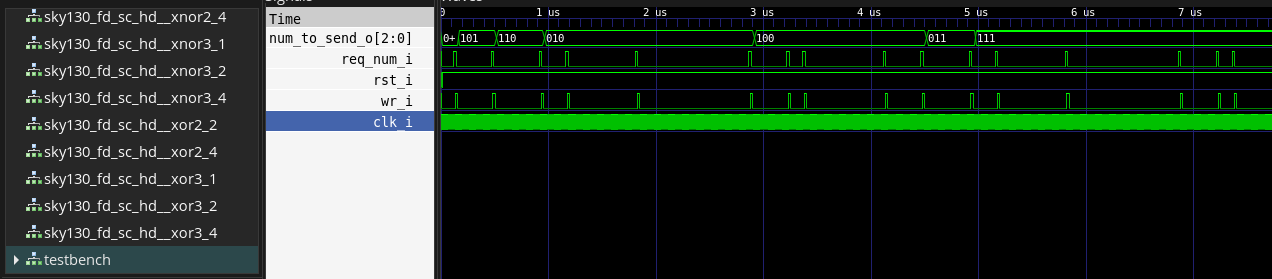
\includegraphics[width=1.0\textwidth]{../../diagrams/waveform_cpa.png}}
		\caption{Waveform da Simulação} 
		\label{fig:waveform}
	\end{figure}
	
	\vfill
	\begin{center}
		\textbf{Metodologia:} Design Síncrono com validação via Handshake e Testbenchs Automatizados.
	\end{center}
	
\end{document}